%\documentclass[11pt,a4paper]{article}
%\usepackage{fullpage}
%\usepackage{beamerarticle}
%\documentclass[handout,xcolor=pdftex,dvipsnames,table]{beamer}
\documentclass[hyperref={unicode=true}]{beamer}

%\usepackage{pgfpages} 
%\pgfpagesuselayout{resize}[a4paper,border shrink=5mm,landscape] 

\usepackage[utf8]{inputenc}
\usepackage[russian]{babel}
\usepackage{../clrscode3e} 
%\usepackage[all]{xy}
\usepackage{colortbl}
%\usepackage{xcolor}
%\usepackage{pstricks, pst-tree, pst-node}
\usepackage{epsfig}
\usepackage{multicol}
%\usepackage{listings}

\definecolor{orange}{cmyk}{0,0.52,1,0}

%\usepackage{beamerthemesplit}

\AtBeginSubsection[]
{
  \begin{frame}<beamer>{Раздел}
    \tableofcontents[currentsection,currentsubsection]
  \end{frame}
}


\newtheorem{rtheorem}{Теорема} 
\newtheorem{rconsequence}{Следствие} 
%default}
%themesplit}

\title{Поиск образца в строке}
\subtitle{Дискретный анализ 2012/13}
\author{Андрей Калинин, Татьяна Романова}
\date{15 октября 2012\,г. }
\usetheme{default}
%\usefonttheme{serif}
\usefonttheme[onlymath]{serif}
%\usefonttheme{professionalfonts}
%\usetheme{default} 


\begin{document}

\frame{\titlepage}

%\section[Содержание]{}
\frame{\tableofcontents}

%\section{Литература}
\frame
{
  \frametitle{Литература}

  \begin{itemize}
  \item Дэн Гасфилд, <<Строки деревья и последовательности в алгоритмах:
    Информатика и вычислительная биология>>, 2003. Глава 1, <<Точное
    совпадение>>, глава 2, <<Точное совпадение: классические
    методы>>, глава 3 <<Более глубокий взгляд>>, стр. 19--94. 
  \item Билл Смит, <<Методы и алгоритмы вычислений на строках>>,
    2006. 
  \end{itemize}
}

\section{Введение}

\subsection{Основные определения}

\frame{
  \frametitle{Строка}
  \begin{enumerate}
  \item Строка $S$ --- упорядоченный список символов, записанный подряд
    слева направо. 
  \item $S(i)$ --- $i$-й символ строки $S$.
  \item $S[i..j]$ --- сплошная подстрока, начинающаяся в позиции с
    $i$ и заканчивающаяся в позиции $j$. $S[i..j]$ пуста, если $i > j$.
  \item $|S|$ --- количество символов в строке $S$.
  \item $S[1..i]$ --- префикс строки $S$.
  \item $S[i..|S|]$ --- суффикс строки $S$.
  \item Собственные суффикс и префикс строки $S$ не пусты и не
    совпадают со строкой. 
  \end{enumerate}
}

\frame{
  \frametitle{Строки и последовательности}
  \begin{itemize}
    \item Строка и последовательность --- синонимы. 
    \item Подстрока и подпоследовательность --- разные
      термины: подстрока является подпоследовательностью, обратное не
      обязательно. В подстроке символы исходной строки должны идти
      подряд, в подпоследовательности должен только соблюдаться
      порядок.  
    \item Для $ababac$: $aba$ --- подстрока, $abc$ --- подпоследовательность.
  \end{itemize}
}

\frame{
  \frametitle{Соглашения}
  \begin{itemize}
    \item $S$ --- любая строка.
    \item $P$ --- образец. 
    \item $T$ --- текст. 
    \item Строчные греческие буквы ($\alpha$, $\beta$, $\gamma$,
      $\delta$ и т.д.) --- переменные строки. 
    \item Строчные латинские буквы ($x$, $y$, $z$ и т.д.) ---
      отдельные переменные символы. 
    \item $\Sigma$ --- алфавит. 
  \end{itemize}
}

\subsection{Постановка задачи}

\frame{
  \frametitle{Точное совпадение}
  Заданы:
  \begin{enumerate}
  \item Строка $P$ --- образец или паттерн. 
  \item Строка $T$ --- текст. 
  \end{enumerate}
  Необходимо отыскать все вхождения образца $P$ в текст $T$.

  Для $P=aba$ и $T=bbabaxababay$ образец входит в текст начиная с
  позиций 3, 7, 9. 
}

\subsection{Очевидный метод}

\begin{frame}
  \frametitle{Алгоритм}
  \begin{codebox}
    \Procname{$\proc{Naive-Pattern-Search}(P,T)$}
    \li $n \gets |P|$
    \li $m \gets |T|$
    \li \For $i \gets 1$ \To $m-n+1$ 
    \li \Do $j \gets 1$
    \li \While $j \leq n$ \func{and} $P(j) \isequal T(j)$ 
    \li \Do $j \gets j+1$ \End
    \li \If $j \isequal n+1$ \Then 
    \li \Comment Вхождение образца в позиции $i$.
    \End
    \End
  \end{codebox}
\end{frame}

\begin{frame}
  \frametitle{Время работы}
  \begin{enumerate}
    \item Худший случай: $P$ и $T$ состоят из одного и того же
      повторяющегося символа. 
    \item Тогда выполняется $n\times(m-n+1)$ сравнений. 
    \item $P=aaa$ и $T=aaaaaaaaaa$, то $n=3$ и $m=10$, выполняется 24
      сравнения. 
  \end{enumerate}
\end{frame}

\begin{frame}
  \frametitle{Идеи по улучшению}
  \begin{itemize}
    \item Не сравнивать два раза одни и те же символы из текста,
      использовать информацию о результатах предыдущих сравнений с
      образцом.
    \item Предварительно обрабатывать образец, выявлять в нём
      структуру, закономерности. 
    \item Сдвигать образец более чем на один символ. 
    \item Возможны линейный и сублинейный алгоритмы поиска образца. 
  \end{itemize}
\end{frame}

\section{Предварительная обработка образца}

\subsection{$Z$-блоки}

\frame{
  \frametitle{$Z_i(S)$}
  
  Для данной строки $S$ и позиции $i>1$ определяется величина $Z_i(S)$
  как длина наибольшего префикса $S[i..|S|]$, совпадающего с префиском
  $S$.
  \\~\\
  Если $S=aabcaabxaaz$, то
  \begin{itemize}
    \item $Z_5(S)=3$ ($aabc\ldots aabx\ldots$).
    \item $Z_6(S)=1$ ($aa\ldots ab\ldots$).
    \item $Z_7(S)=Z_8(S)=0$.
    \item $Z_9(S)=2$ ($aab\ldots aaz$).
  \end{itemize}
}

\frame{
  \frametitle{$Z$-блок}
  Для любой позиции $i>1$
  \begin{enumerate}
    \item в которой $Z_i>0$, $Z$-блок это
      интервал, начинающийся в $i$ и кончающийся в позиции
      $i+Z_i-1$.
    \item $r_i$ --- крайний правый конец $Z$-блоков, начинающихся не
      позднее $i$. Или 
      \[r_i = \displaystyle\max_{1<j\leq i}\{j+Z_j-1\}\]
    \item $l_i$ --- значение, на котором достигается этот максимум
      (т.е. $Z_{l_i}$ заканчивается в $r_i$). Или 
\[l_i = \displaystyle\arg\max_{1<j\leq i}\{j+Z_j-1\} \]
  \end{enumerate}
}

\frame{
  \frametitle{$Z$-блоки}
%\includegraphics[width=\textwidth]{zblocks.1.eps}
  Позиция $i$ находится внутри двух $Z$-блоков, выбирается с
  максимальной правой границей, $r_i$. \\
  ~\\
~\\
~\\
~\\
  \includegraphics[scale=1.0]{substring-search.1.eps}
}

\subsection{Построение $Z$-блоков за линейное время}

\frame{
  \frametitle{Основные идеи}
  \begin{enumerate}
    \item $Z_2$, $r_2$ и $l_2$ строятся непосредственным сравнением
      строк $S$ и $S[2..|S|]$. 
    \item Допустим, $Z_i$ получено для всех $1< i \leq k-1$ и нужно
      найти $Z_k$.
    \item Известно, что $S[k..r_{k-1}]$ совпадает с некоторой строкой
      из префикса $S$, начиная с $k'=k-l_{k-1}+1$. 
    \item Тогда, исходя из значения $Z_{k'}$, можно пропустить прямое
      сравнение символов до $r_{k-1}$. 
    \item Тем самым, ни один символ обрабатываемой строки никогда не
      будет сравниваться дважды.  
  \end{enumerate}
}

\frame{
  \frametitle{Подстрока $\beta$}
  Обрабатывается $k$-й символ, $\alpha$ начинается с $l$ и кончается в
  $r$, длина блока $Z_l$ символов, та же строка $\alpha$ располагается
  в префиксе строки $S$. Тогда в префиксе позиции $k$
  соответствует позиция $k' = k-l+1$, где находится
  подстрока $\beta$:\\
  ~\\
~\\
~\\
  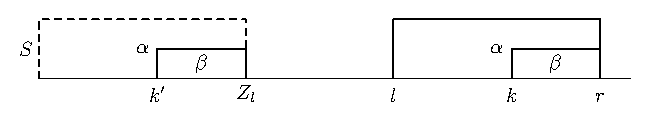
\includegraphics[scale=1.0]{substring-search.2.eps}
}


\frame{
  \frametitle{Алгоритм}
  \begin{codebox}
    \Procname{$\proc{Build-ZBlocks}(S)$}
    \li $r \gets 0$
    \li \For $1 < k \leq |S|$
    \li \Do \If $k>r$ \Comment Случай 1
    \li \Then  $Z_k =\proc{Common-Prefix-Length}(S,S[k..|S|])$
    \li \If $Z_k > 0$ 
    \li \Then $r\gets k+Z_k-1$,  $l \gets k$ \End
    \li \Else $k' \gets k -l+1$ 
    \li \If $Z_{k'}< |\beta|$ \Comment $\beta$ --- строка в $S[k..r]$ и $S[k'..Z_l]$
    \li \Then $Z_k=Z_{k'}$ \Comment Случай 2а
    \li \Else $q \gets r + \proc{Common-Prefix-Length}$ \Comment
    Случай 2б
    \zi $(S[|\beta|+1..|S|],S[r+1..|S|])$
    \li $Z_k \gets q-k+1$, $r \gets q$, $l \gets k$
    \End
    \End
  \end{codebox}
}


\frame{
  \frametitle{$Z_{k'}<|\beta|$}
  $Z$-блок, начинающийся в $k'$, короче $\beta$. Отсюда $Z_k$
  присваивается значение $Z_{k'}$:\\
  ~\\
  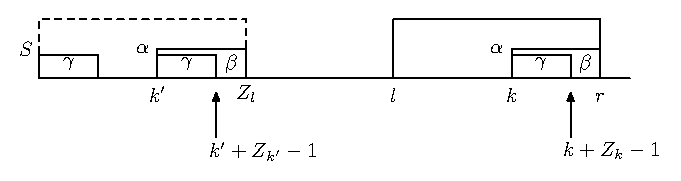
\includegraphics[scale=1.0]{substring-search.3.eps}
}

\frame{
  \frametitle{$Z_{k'}\geq |\beta|$}
  $Z$-блок, начинающийся в $k'$, длиннее $\beta$. Следовательно, $Z_k$
  как минимум равен $r-k+1$, дальше нужно непосредственно сравнить
  подстроки $S[r+1..|S|]$ и $S[Z_l..|S|]$ для вычисления точного
  значения $Z_k$:\\
  ~\\
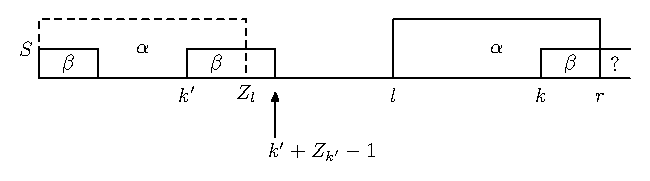
\includegraphics[scale=1.0]{substring-search.4.eps}
}

\frame{
  \frametitle{Пример выполнения алгоритма}
  \begin{tabular}{|c|c|c|c|c|c|c|c|c|c|c|c|}
    \hline
    $k$ & 1 & 2 & 3 & 4 & 5 & 6 & 7 & 8 & 9 & 10 & 11 \\
    \hline
    $S$ & a & a & b & c & a & a & b & x & a & a & z \\
    $Z_k$&  & \onslide<2->{1} & \onslide<3->{0} &
    \onslide<4->{0} & \onslide<5->{3} & \onslide<6->{1} &
    \onslide<7->{0} & \onslide<8->{0} & \onslide<9->{2} & 
    \onslide<10->{1} & \onslide<11->{0}\\

    $r$  & 0& \onslide<2->{2} & \onslide<3->{2} &
    \onslide<4->{2} & \onslide<5->{7} & \onslide<6->{7} &
    \onslide<7->{7} & \onslide<8->{7} & \onslide<9->{10} &
    \onslide<10->{10} & \onslide<11->{10} \\

    $l$  &  & \onslide<2->{2} & \onslide<3->{2} &
    \onslide<4->{2} & \onslide<5->{5} & \onslide<6->{5} &
    \onslide<7->{5} & \onslide<8->{5} & \onslide<9->{9} & 
    \onslide<10->{10} & \onslide<11->{10}\\

    \hline
  \end{tabular}
  \\~\\~\\
  \only<2>{$k=2$: $Z_2$ получен прямым сравнением.}
  \only<3>{$k=3$: Так как $r$ меньше 3, то опять выполняется
    непосредственное сравнение префиксов начиная с 3-й позиции.}
  \only<4>{$k=4$: $r < 4$, вычисляем $Z_4$ прямым сравнением.}
  \only<5>{$k=5$: $r < 5$, сравниваем префиксы. На этот раз $Z_5=3$,
    заполняем значения $l=k=5$ и $r=k+Z_5-1=7$.}
  \only<6>{$k=6$: $r > 6$, $k'=2$ и $Z_2=1$, т.е. правая граница $Z$-блока
   заканчивается раньше, чем $Z_5$ символов от начала $S$,
   следовательно $Z_6=Z_2=1$ без каких либо сравнений.}
 \only<7>{$k=7$: Аналогично, $Z_7=Z_3=0$ без выполнения сравнений символов.}
 \only<8>{$k=8$: $r < 8$, выполняем непосредственное сравнение. }
 \only<9>{$k=9$: Непосредственным сравнением находим $Z_9=2$, заполняем
   $r=10$ и $l=9$.}
 \only<10>{$k=10$: Т.к. $Z_2=1$, то $Z_{10}$ как минимум равен 1 и  $Z$-блок заканчивается на границе
   проверенных данных, нужно попытаться сравнить символы 11-й и
   2-й. Несмотря на то, что они не равны, модифицируются переменные
   $r$ и $l$.}
 \only<11>{$k=11$: Непосредственным сравнением получаем $Z_{11}=0$.}
 \vfill
}

\frame{
  \frametitle{Корректность вычисления $Z_k$}
  \begin{rtheorem}
    При использовании одной итерации алгоритма $\proc{Build-ZBlocks}$ значения $Z_k$
    корректно вычисляются и переменные $r$ и $l$ корректно
    обновляются. 
  \end{rtheorem}
  \begin{rconsequence}
    Повторное применение алгоритма для каждой позиции $k>2$ корректно
    находит все значения $Z_k$.
  \end{rconsequence}
}
\frame{
  \frametitle{Корректность вычисления $Z_k$: доказательство}
  \begin{proof}
    \begin{enumerate}
      \item Случай 1, $k>r$: $Z_k$ вычисляется
        непосредственно. Замена $r$ корректна, т.к. нет
        ни одного $Z$-блока, кончающего-ся в $k$ или после неё. 
      \item Случай 2а, $Z_{k'}<|\beta|$: Если $Z_k\geq |\beta|$, то 
        $S(k'+Z_{k'}) = S(k+Z_{k}) = S(1+Z_{k'})$, что противоречит
        корректности вычисления $Z_{k'}$. $k+Z_k -1<r$, т.е. $r$ и $l$
        не меняются.
      \item Случай 2б, $Z_{k'}\geq|\beta|$: $\beta$ является префиксом
        $S$, продолжение вычисляется непосредственно. $k+Z_k-1\geq r$,
        следовательно меняются $r$ и $l$.
    \end{enumerate}
  \end{proof}
}

\frame{
  \frametitle{Линейность алгоритма построения $Z$-блоков}
  \begin{rtheorem}
    Все значения $Z_k(S)$ вычисляются алгоритмом
    $\proc{Build-ZBlocks}$ за время $O(|S|)$.
  \end{rtheorem}
  \begin{proof}
    \begin{enumerate}
      \item Число итераций: $|S|$.
      \item При выполнении сравнений несовпадение завершает итерацию,
        т.е. количество несовпадений $|S|$.
      \item $\forall k:$ $r_k \geq r_{k-1}$. Если было $q > 0$
        совпадений, то $r_k \geq r_{k-1}+q$. Кроме того, $r_k \leq
        |S|$ и сравнения выполняются только когда $k>r$, следовательно
        число совпадений не превосходит $|S|$.
    \end{enumerate}
  \end{proof}
}

\subsection{Поиск с использованием $Z$-блоков}

\frame{
  \frametitle{Простейший алгоритм линейного поиска}
  \begin{itemize}
  \item $S=P\$T$, где $\$$ --- символ, отсутствующий в $P$ и $T$.
  \item $|P|=n$, $|T|=m$, $n\leq m$, $\Rightarrow$ $|S|=n+m+1=O(m)$.
  \item Вычисляем $Z_i(S)$ для $2 \leq i \leq n+m+1$, $Z_i\leq n$.
  \item Для всех значений $i>n+1$, для которых $Z_i(S)=n$, есть
    вхождение $P$ в $T$ в позиции $i-(n+1)$.  
  \item И наоборот: если есть вхождение $P$ в $T$ в, то $Z_{n+1+j}=n$.
  \item $O(n+m) = O(m)$.
  \end{itemize}
}

\frame{
  \frametitle{Свойства алгоритма}
  \begin{itemize}
    \item Время выполнения $O(m)$.
    \item Требуется дополнительная память размера $O(n)$ ($Z$-блоки
      для образца).
    \item Алфавитно-независимый метод: нужна только операция сравнения
      символов, не нужно даже знать размерность алфавита. 
  \end{itemize}
}

\frame{
  \frametitle{Зачем продолжать?}
  \begin{itemize}
    \item Поиск набора образцов в тексте. 
    \item Алгоритмы реального времени. 
    \item Сублинейное время работы.
    \item Время работы, пропроциональное длине образца (суффиксные
      деревья). 
  \end{itemize}
}

\section{Алгоритм Кнута-Морриса-Пратта}

\subsection{Основной алгоритм}

\frame{
  \frametitle{Общая идея}
  \begin{itemize}
  \item Образец прикладывается к тексту как в очевидном (<<наивном>>)
    алгоритме. 
  \item Выполняются сдвиги образца более, чем на один символ. 
  \item Для выполнения сдвигов исследуются суффиксы и префиксы
    подстрок образца. 
  \item Сравнение продолжается с той же позиции в тексте, на котором
    закончилась предыдущая итерация. 
  \item Для $P=abcxabcde$ и несовпадении в 8-й позиции можно сдвинуть
    $P$ на 4 места вне зависимости от текста $T$.
  \end{itemize}
}

\begin{frame}[fragile]
  \frametitle{Пример}
\begin{semiverbatim}
....a\alert<2>{b}\alert<3>{c}\alert<4>{x}\alert<5->{abc}\alert<1>{?}....
\only<2->{ }\only<3->{ }\only<4->{ }\only<5->{ }    \alert<2-5>{a}\alert<5->{bc}xabc\alert<1>{d}e
\end{semiverbatim}
\end{frame}

\frame{
  \frametitle{$sp_i$ и $sp'_i$}
  \begin{itemize}
    \item $sp_i(P)$ --- длина наибольшего собственного суффикса
      $P[1..i]$, совпадающим с префиксом $P$.
    \item $sp'_i(P)$ --- то же самое с дополнительным условием 
      $P(i+1) \neq P(sp'_i+1)$.
    \item $sp'_i(P) \leq sp_i(P)$
  \end{itemize}
}

\frame{
  \frametitle{Примеры $sp_i$  и $sp'_i$}
  \begin{tabular}{|cccccccccccc|}
    \hline $i$  & 1 & 2& 3& 4& 5& 6& 7& 8& 9&10&11 \\
    \hline \rowcolor{orange} $P$    & a & b& c& a& e&a&b&c&a&b&d \\
    \hline $sp_i$ & 0 & 0& 0& 1& 0&1&2&3&4&2&0 \\
    $sp'_i$& 0 & 0& 0& 1& 0&0&0&0&4&2&0 \\ 
    \hline
    
  \end{tabular} \\
  ~ \\
  ~ \\
  \begin{tabular}{|ccccccccccccc|}
    \hline  $i$      & 1 & 2& 3& 4& 5& 6& 7& 8& 9&10&11&12 \\
    \hline  \rowcolor{orange} $P$  &b&b&c&c&a&e&b&b&c&a&b&d \\
    \hline $sp_i$ &0&1&0&0&0&0&1&2&3&0&1&0 \\
     $sp'_i$&0&1&0&0&0&0&0&1&3&0&1&0\\
    \hline
  \end{tabular}
}

\frame{
  \frametitle{Правило сдвига Кнута-Морриса-Пратта}
  \begin{itemize}
    \item $P(i+1) \neq T(k)$: сдвиг выполняется таким образом, что 
      $P[1..sp'_i] \rightarrow T[k-sp'_i..k-1]$, т.е. образец
      смещается  вправо на $i-sp'_i$ позиций. 
    \item При обнаружении вхождения: сдвиг на $n-sp'_n$ мест.
    \item В следующем сравнении будут участвовать символы $T(k)$ и
      $P(sp'_i+1)$. 
  \end{itemize}
}


\frame{
  \frametitle{Корректность}
  \begin{rtheorem}
    После несовпадения в позиции $i+1$ образца $P$ и сдвига на
    $i-sp'_i$ мест вправо левые $sp'_i$ символов $P$ гарантировано
    совпадут со своими парами в $T$.
  \end{rtheorem}
  \begin{rtheorem}
    Для любого выравнивания $P$ с $T$ если $P[1..i] = T[k-i..k-1]$ и 
    $P(i+1) \neq T(k)$, то $P$ может быть сдвинуто на $i-sp'_i$
    позиций вправо без пропуска вхождений $P$ в $T$.
  \end{rtheorem}
}

\frame{
  \frametitle{Отсутствие пропусков}
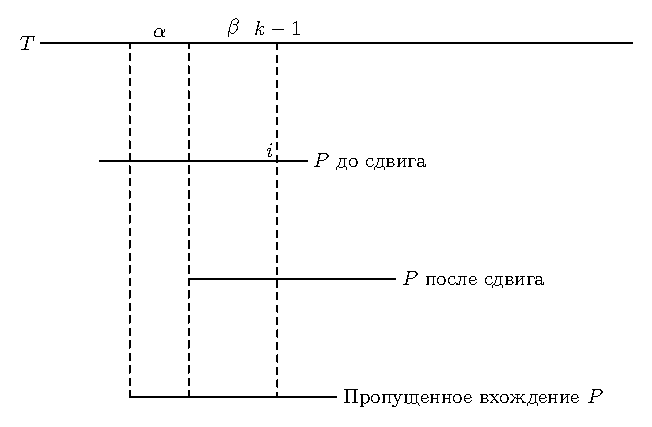
\includegraphics[scale=1.0]{substring-search.5.eps}
}

\frame{
  \frametitle{Линейность}
  \begin{rtheorem}
    В методе Кнута-Морриса-Пратта число сравнений символов не
    превосходит $2m$.
  \end{rtheorem}
  \begin{proof}
    \begin{itemize}
      \item Фазы сравнения/сдвига: некоторое количество сравнений и
        сдвиг образца. 
      \item В каждой фазе не более одного сравнения с символом из $T$,
        который уже сравнивался. 
      \item Количество сравнений $m+s$, где $s$ --- число сдвигов;
        т.к. $s<m$, то общее число сравнений меньше $2m$.
    \end{itemize}
  \end{proof}
}


\frame{
  \frametitle{Связь $sp'_i$ с $Z$-блоками}
  \begin{enumerate}
    \item $j$ отображается в $i$, если $i=j+Z_j(P)-1$.
    \item $sp'_i=Z_j=i-j+1$, где $j$ --- наименьший индекс
      отображаемый в $i$. Если такого $j$ нет, то $sp'_i=0$.
    \item $sp_i=i-j+1$, где $j$ --- наименьший индекс $1<j\leq i$,
      отображаемый в $i$ или дальше. Если такого $j$ нет, то
      $sp_i=0$. 
  \end{enumerate}
}

\frame{
  \frametitle{Примеры $sp_i$  и $sp'_i$ с $Z$-блоками}
  \begin{tabular}{|cccccccccccc|}
    \hline $i$  & 1 & 2& 3& 4& 5& 6& 7& 8& 9&10&11 \\
    \hline \rowcolor{orange} $P$    & a & b& c& a& e&a&b&c&a&b&d \\
    \hline $sp_i$ & 0 & 0& 0& 1& 0&1&2&3&4&2&0 \\
    $sp'_i$& 0 & 0& 0& 1& 0&0&0&0&4&2&0 \\ 
    $Z_i$  & &0&0&1&0&4&0&0&2&0&0 \\
    \hline
    
  \end{tabular} \\
  ~ \\
  ~ \\
  \begin{tabular}{|ccccccccccccc|}
    \hline  $i$      & 1 & 2& 3& 4& 5& 6& 7& 8& 9&10&11&12 \\
    \hline  \rowcolor{orange} $P$  &b&b&c&c&a&e&b&b&c&a&b&d \\
    \hline $sp_i$ &0&1&0&0&0&0&1&2&3&0&1&0 \\
     $sp'_i$&0&1&0&0&0&0&0&1&3&0&1&0\\
     $Z_i$& &1&0&0&0&0&3&1&0&0&1&0 \\
    \hline
  \end{tabular}
}

\frame{
  \frametitle{Вычисление $sp'_i$ и $sp_i$}
  \begin{codebox}
    \li \For $i \gets 1$ \To $n$ 
    \li \Do $sp'_i \gets 0$ \End
    \li \For $j \gets n$ \Downto $2$
    \li \Do $i \gets j+Z_j(P)-1$
    \li $sp'_i \gets Z_j(P)$
    \End
    \li $sp_n \gets sp'_n$
    \li \For $i \gets n-1$ \Downto $2$
    \li \Do $sp_i \gets \max\{sp_{i+1}-1, sp'_i\}$
    \End
  \end{codebox}
}


\frame{
  \frametitle{Функция неудачи}
  \begin{itemize}
  \item $F'(i) = sp'_{i-1}+1$.
  \item $F(i) = sp_{i-1}+1$.
  \item Функция неудачи показывает, какой символ образца нужно
    сравнивать с текущим символов текста при несовпадении в $P(i)$.
  \end{itemize}
}

\frame{
  \frametitle{Алгоритм Кнута-Морриса-Пратта}
  \begin{codebox}
    \zi \Comment Обработать $P$ и найти $F'(k)$ для $1 \leq k \leq n+1$.
    \li $c \gets 1$, $p \gets 1$
    \li \While $c+n-p \leq m$ 
    \li \Do \While $P(p) \isequal T(c)$ \func{and} $p \leq n$ 
    \li \Do $p \gets p+1$, $c \gets c+1$ \End
    \li \If $p \isequal n+1$ 
    \li \Then \Comment Вхождение $P$ в $T$ в позиции $c-n$. \End
    \li \If $p \isequal 1$ 
    \li \Then $c \gets c+1$ \End
    \li $p \gets F'(p)$ \End
  \end{codebox}
}

\frame{
  \frametitle{Выводы}
  \begin{itemize}
    \item Сдвиги выполняются больше чем на один символ. 
    \item Текст обрабатывается последовательно, нет возвратов. 
    \item Линейный (но не сублинейный) алгоритм. 
    \item Нет зависимости от алфавита. 
  \end{itemize}
}

\subsection{Алгоритм реального времени}

\frame{
  \frametitle{Алгоритмы реального времени}
  \begin{itemize}
  \item Константное время между проверками любых позиций текста.
  \item Более строгое понятие, чем линейный алгоритм. 
  \item Предыдущий алгоритм линейный, но не реального времени:
    неизвестно сколько времени потребуется на выполнение сдвига у
    определённой позиции, может быть 1 такт, а может $|P|$ тактов.  
  \item Для преобразования нужно рассчитать $sp'_i$ для каждого
    символа алфавита, с которым происходит сравнение. 
  \end{itemize}
}

\frame{
  \frametitle{$sp'_{(i,x)}$}
  \begin{itemize}
    \item $x \in \Sigma$. 
    \item $sp'_{(i,x)}$ --- длина наибольшего собственного суффикса
      $P[1..i]$, совпадающий с префиксом $P$, при условии что
      $P(sp'_i+1)=x$.
    \item Можно сформулировать правило сдвига, при котором или
      гарантируется совпадение $T(k)=P(sp'_{i,x}+1)$, или гарантируется
      отсутствие префикса, продолжающегося символом $T(k)$.
    \item Тогда никакой символ $T$ не проверяется больше одного раза. 
  \end{itemize}
}

\frame{
  \frametitle{Вычисление $sp'_{(i,x)}$}
  Если  $P(i+1)\neq x$, то $sp'_{(i,x)}=i-j+1$, где $j$ --- наименьшая
  позиция, такая что $j$ отображается в $i$ и $P(Z_j+1)=x$. Если
  такого $j$ нет, то $sp'_{(i,x)}=0$.\\
  \begin{codebox}
    \li \For $i \gets 1$ \To $n$ 
    \li \Do \For $x \in \Sigma$ 
    \li \Do $sp'_{(i,x)} \gets 0$ \End \End
    \li \For $j \gets n$ \Downto $2$
    \li \Do $i \gets j+Z_j(P)-1$, $x \gets P(Z_j)+1$,
    $sp'_{(i,x)}\gets Z_j$ \End
  \end{codebox}
}

\section{Алгоритм Бойера-Мура}

\subsection{Основная идея}

\frame{
  \frametitle{Основная идея}
  \begin{itemize}
    \item Образец последовательно прикладывается к тексту, сравнение
      идёт справа налево. 
    \item Правило сдвига по плохому символу. 
    \item Правило сдвига по хорошему суффиксу. 
    \item Обычно проверяется не больше, чем $m+n$ символов, линейное
      время в худшем случае (сильное правило хорошего суффикса) и
      ожидаемое сублинейное время. 
  \end{itemize}
}

\frame{
  \frametitle{Функция $R(x)$}
  \begin{itemize}
    \item Для каждого символа алфавита $x$ пусть $R(x)$ --- позиция
      крайнего правого вхождения $x$ в $P$. Если $x$ в $P$ не входит,
      $R(x)=0$.
    \item Время подготовки таблицы для $R(x)$: $O(n)$.
    \item Например: $abad$, $R(b)=2$, $R(a)=3$. Соответственно, если
      при первом сравнении образца в тексте был обнаружен символ $b$,
      то образец можно сдвинуть на $|P|-R(b)=4-2=2$ символа.  
  \end{itemize}
}

\frame{
  \frametitle{Правило сдвига по плохому символу}
  \begin{itemize}
    \item Правый символ $P$ приложен к позиции $q$ в тексте. 
    \item $P(n)=T(q)$, $P(n-1)=T(q-1)$, ...
    \item $P(n-i) \neq T(k)$; $k=q-i$.
    \item Тогда $P$ можно сдвинуть вправо на $\max\{1, i-R(T(k))\}$
    мест. 
    \item Если крайнее правое вхождение в $P$ символа $T(k)$
      занимает позицию $j<i$, то $P$ сдвигается так, чтобы символ $j$
      поравнялся с символом $k$ в $T$. В противном случае, $P$
      сдвигается на одну позицию. 
    \item Правило эффективно при несовпадениях, близких к правому
      концу $P$.
  \end{itemize}
}

\frame{
  \frametitle{Расширенное правило плохого символа}
  \begin{itemize}
  \item Несовпадение в позиции $i$ образца $P$.
  \item $x$ --- несовпадающий символ в $T$.
  \item Нужно совместить с этим $x$ ближайшее вхождение $x$ в $P$
    слева от $i$. 
  \item Для $abad$ $R(a,4)=3$ и $R(a,2)=1$.
  \end{itemize}
}

\frame{
  \frametitle{Реализация расширенного правила}
  \begin{itemize}
  \item Таблица размером $n\times|\Sigma|$.
  \item Для каждого символа алфавита $x$ хранить список позиций в $P$,
    расположенных по убыванию. Например, для $P=abacbabc$ и символа
    $a$ получится список $\langle 6, 3, 1 \rangle$.
  \end{itemize}
}

\frame{
  \frametitle{Свойства правила}
  \begin{itemize}
  \item Высокая эффективность в практических условиях, для текстов с
    большими размерами алфавитов (английский текст). 
  \item Для маленьких алфавитов --- хуже.
  \item Не гарантирует линейности. 
  \end{itemize}
}

\subsection{Правило хорошего суффикса}

\frame{
  \frametitle{Сдвиг по хорошему суффиксу}
  Символ $x$ из $T$ не совпал с $y$ из $P$. По сильному правилу
  хорошего суффикса обеспечивается сдвиг таким образом, чтобы $\beta'$
  приложилось к $\beta$, где $z \neq y$.\\
~\\
  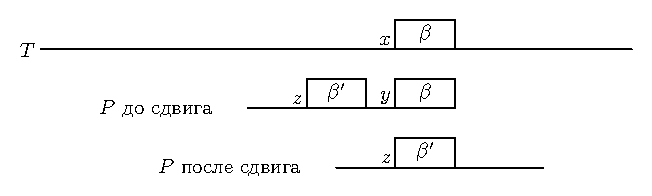
\includegraphics[scale=1.0]{substring-search.6.eps}
}

\frame{
  \frametitle{Cильное правило хорошего суффикса}
  \begin{itemize}
  \item $P$ приложена к $T$. $\beta$ --- суффикс $P$, совпадает с
    подстрокой $T$, символ $y$ не совпадает с $x$ из $T$.
  \item Если существует $\beta'$, самая правая копия $\beta$ в $P$ такая,
    что предшествующий ей символ $z \neq y$, то нужно обеспечить такой
    сдвиг образца, чтобы $\beta'$ приложилась к $\beta$.
  \item В противном случае нужно сдвинуть образец на наименьший сдвиг,
    при котором собственный префикс сдвинутого образца совпадает с
    суффиксом вхождения $P$ в~$T$.
  \item Если и такой сдвиг невозможен, то выполняется свдиг $P$ на $n$
    позиций. 
  \end{itemize}
}

\begin{frame}[fragile]
  \frametitle{Пример}
\begin{columns}
\begin{column}{0.5\textwidth}
\begin{semiverbatim}
123456789012345678
prstabstu\alert<1>{b}\alert<2>{ab}vqxrst
  qc\alert<2>{ab}dab\alert<1>{d}\alert<2>{ab}
  1234567890
\end{semiverbatim}
\end{column}
\begin{column}{0.5\textwidth}
\begin{semiverbatim}
\uncover<3->{
123456789012345678
prstabstub\alert<3>{ab}vqxrst
        qc\alert<3>{ab}dabdab
        1234567890
}
\end{semiverbatim}
\end{column}
\end{columns}
\only<1>{$P(8) \neq T(10)$.}
\only<2>{$\beta = ab$, $\beta' = P[3..4]$.}
\only<3>{$P[3..4] = T[11..12]$.}
\end{frame}

\frame{
  \frametitle{Корректность правила хорошего суффикса}
  \begin{rtheorem}
    Использование правила хорошего суффикса никогда не сдвинет $P$ за его вхождение в $T$.
  \end{rtheorem}
  \begin{proof}
    \begin{itemize}
    \item До сдвига правый конец $P$ стоял у позиции $k$ в $T$ и
      сдвиг произошёл к позиции $k'$. 
    \item Предположим, что в позиции $k < l < k'$ заканчивалось
      пропущенное вхождение $P$.
    \item Тогда в $P$ должна быть либо более близкая копия $\beta$ или
      более длинный префикс совпадал бы с суффиксом $\beta$.
    \end{itemize}
  \end{proof}
}

\frame{
  \frametitle{Пропущенное вхождение в $l$}
  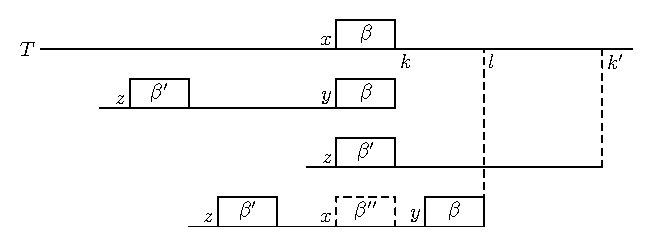
\includegraphics[scale=1.0]{substring-search.7.eps}
}

\frame{
  \frametitle{Слабое правило хорошего суффикса}
  \begin{itemize}
    \item Было сформулировано в оригинальном алгоритме. 
    \item Аналогично сильному правилу, но не требует разных символов перед
      $\beta$ и $\beta'$.
    \item Не даёт возможность получить линейную наихудшую оценку. 
  \end{itemize}
}
\subsection{Реализация}

\frame{
  \frametitle{$L(i)$, $L'(i)$, $N_i(P)$}
  Для каждого i:
  \begin{itemize}
  \item $L(i) < n$ --- наибольшая позиция, такая что $P[i..n]$
    совпадает с суффиксом $P[1..L(i)]$. 
  \item $L'(i) < n$ --- наибольшая позиция, такая что $P[i..n]$
    совпадает с суффиксом $P[1..L'(i)]$, а символ, предшествующий ему,
    не равен $P(i-1)$.
  \item $N_i(P)$ --- длина наибольшего суффикса $P[1..i]$, который
    является также суффиксом $P$.
  \item Если $P^r$ --- реверс $P$, то $N_i(P)=Z_{n-i+1}(P^r)$,
    т.е. $N_i(P)$ вычисляется при помощи $\proc{Build-ZBlocks}$.
  \end{itemize}
%  Если $P=cabdabdab$, то $L(8)=6$, $L'(8)=3$, $N_3(P)=2$ и $N_6(P)=5$.
}

\frame{
  \frametitle{Вычисление $L(i)$ и $L'(i)$}
  \begin{eqnarray*}
  L(i) &=& \max\left\{1\leq j < n \Big| N_j(P)\geq
    \left|P[i..n]\right|=n-i+1\right\} \\
  L'(i) &=& \max\left\{1\leq j<n\Big|N_j(P) = n-i+1\right\}
  \end{eqnarray*}
  
  \begin{columns}
    \begin{column}{.4\textwidth}
  \begin{codebox}
%    \Procname{$\proc{Build-L}(S)$}
    \li \For $i \gets 1$ \To $n$
    \li \Do $L'(i) \gets 0$ \End
    \li \For $j \gets 1$ \To $n-1$
    \li \Do $i \gets n-N_j(P)+1$
    \li $L'(i) \gets j$
    \End
    \li $L(2) \gets L'(2)$
    \li \For $i \gets 3$ \To $n$
    \li \Do $L(i) \gets \max\{L(i-1),L'(i)\}$
    \End
  \end{codebox}
  \end{column}
  \begin{column}{.6\textwidth}
  \begin{tabular}{|cccccccccc|}
    \hline $i$ &1&2&3&4&5&6&7&8&9\\
    \hline \rowcolor{orange} $P$ &c&a&b&d&a&b&d&a&b\\
    \hline $L$ &0&0&0&0&6&6&6&6&6\\
    $L'$&0&0&0&0&6&0&0&3&0 \\
    $N$ &0&0&2&0&0&5&0&0&  \\
    \hline
  \end{tabular}

  \end{column}
  \end{columns}
}

\frame{
  \frametitle{$l'(i)$}
  \begin{itemize}
  \item $l'(i)$ --- длина наибольшего суффикса $P[i..n]$, который
    является префиксом $P$, если такой существует. Если его не
    существует, то $l'(i)=0$.
  \item $ l'(i) = \max\left\{1 \leq j \leq |P[i..n]|=n-i+1\Big|N_j(P)=j \right\}$    
  \end{itemize}
  \begin{columns}
    \begin{column}{.4\textwidth}
  \begin{codebox}
    \li $l'(n+1) \gets 0$
    \li \For $i\gets n$ \Downto $1$
    \li \Do $j \gets n-i+1$
    \li \If $N_j(P) \isequal j$
    \li \Then $l'(i) \gets j$ 
    \li \Else $l'(i) \gets l'(i+1)$
    \End \End
  \end{codebox}
  \end{column}
  \begin{column}{.6\textwidth}
  \begin{tabular}{|cccccccccc|}
    \hline 
    $i$ &1&2&3&4&5&6&7&8&9\\
    \hline \rowcolor{orange} 
           $P$ &a&b&a&b&c&a&b&a&b\\
    \hline $l'$&4&4&4&4&4&4&2&2&0\\
           $N$ &0&2&0&4&0&0&2&0& \\
    \hline 
  \end{tabular}
  \end{column}
  \end{columns}
}

\frame{
  \frametitle{Алгоритм Бойера-Мура}
  \begin{codebox}
    \Procname{$\proc{BM-Pattern-Search}(P,T)$}
%    \zi \Comment Вычисление $L'(i)$, $l'(i)$ и $R(x)$
    \li $k \gets n$
    \li \While $k \leq m$
    \li \Do $i\gets n$, $h \gets k$
    \li \While $i>0$ \func{and} $P(i) \isequal T(h)$
    \li \Do $i \gets i-1$, $h \gets h-1$ \End
    \li \If $i \isequal 0$ \Comment Вхождение $P$ в $T$, оканчивающиеся в $k$
    \li \Then $k \gets k + n - l'(2)$
    \li \ElseIf $i \isequal n$
    \li \Then $k \gets k + 1$
    \li \ElseIf $L'(i+1) > 0$
    \li \Then $s \gets n-L'(i+1)$
    \li \Else $s \gets n-l'(i+1)$ \End
    \li $k \gets k + \max\{1, s, i+1-R(x)\}$
    \End
    \End
  \end{codebox}
}

\frame{
  \frametitle{Свойства алгоритма}
  \begin{itemize}
  \item Для слабого правила хорошего суффикса если образец не
    встречается в тексте, то время работы в худшем случае
    $O(nm)$. Однако в среднем --- сублинейное время.  
  \item Сильное правило хорошего суффикса: $O(m)$, не больше $4m$
    сравнений. 
  \item Алфавито-независимый алгоритм (с точностью до организации $R(x)$). 
  \item Доказательство линейности очень сложное, вместо него будет
    разобран алгоритм Апостолико-Джанкарло с простой оценкой
    количества сравнений $2m$ в худшем случае. 
  \end{itemize}
}


\section{Алгоритм Апостолико-Джанкарло}

\subsection{Имитация алгоритма Бойера-Мура}

\frame{
  \frametitle{Основная идея}
  \begin{enumerate}
  \item Имитация алгоритма Бойера-Мура, фазы от $1$ до $q \leq m$. 
  \item Для каждой позиции текста $T$ запоминаются значения 
    $M(j) \leq l$, где $l$ --- количество совпавших символов с
    суффиксом $P$. 
  \item В случае, если сравниваются $P(i)$ и $T(h)$ то по ненулевым значениям
    $N_i$ или $M(h)$ можно предсказать результат этого и последующих сравнений. 
  \end{enumerate}
}

\frame{
  \frametitle{Сравнение $P(i)$ с  $T(h)$}
  $|\alpha|=N_i$, $|\beta|=M(h)>N_i$: строки совпадают на $N_i$
  символов, но дальше различаются. \\
~\\
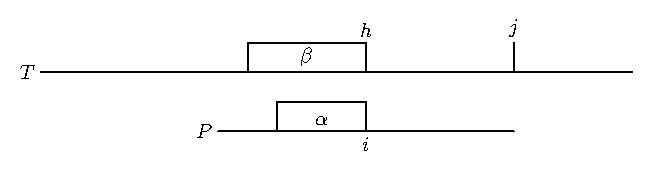
\includegraphics[scale=1.0]{substring-search.8.eps}
}

\frame{
  \frametitle{Одна фаза}
  \begin{enumerate}
    \item $M(h)$ не определено или $M(h)=N_i=0$:
      \begin{itemize}
      \item $T(h)=P(i)$, $i=1$: вхождение образца, $M(j) \leftarrow n$, сдвиг. 
      \item $T(h)=P(i)$, $i>1$: $h \leftarrow h-1$, $i \leftarrow i-1$, повтор. 
      \item $T(h) \neq P(i)$: $M(j)\leftarrow j-h$, сдвиг. 
      \end{itemize}
    \item $M(h) <  N_i$: $i \leftarrow i-M(h)$, $h\leftarrow h-M(h)$,
      повтор. 
    \item $M(h)\geq N_i$ и $N_i = i > 0$: вхождение образца, $M(j)
      \leftarrow j-h$, сдвиг.
    \item $M(h)>N_i$ и $N_i < i$: $P(i-N_i)\neq T(h-N_i)$,
      $M(j)\leftarrow j-h$, сдвиг. 
    \item $M(h)=N_i$ и $0 < N_i < i$: $i\leftarrow i-M(h)$,
      $h\leftarrow h-M(h)$, повтор. 
  \end{enumerate}
}

\frame{
  \frametitle{Корректность алгоритма Апостолико-Джанкарло}
  \begin{rtheorem}
    Используя $M$ и $N$ алгоритм Апостолико-Джанкарло правильно
    находит все вхождения $P$ в $T$.
  \end{rtheorem}
  \begin{proof}
    Алгоритм полностью имитирует алгоритм Бойера-Мура, за исключением
    пропуска некоторых сравнений. 
  \end{proof}
}

\subsection{Линейность}

\frame{
  \frametitle{Вспомогательные определения}
  \begin{itemize}
    \item Если $M(j) \neq 0$, то $[j-M(j)+1..j]$ --- покрытый
      интервал для $j$.
    \item Если для $j'<j$ и $j$ определены покрытые интервалы, то они
      пересекаются, если $j'-M(j')+1 < j-M(j)+1 \leq j'$. 
  \end{itemize}
}

\frame{
  \frametitle{Интервалы}
Непересекающиеся интервалы:\\
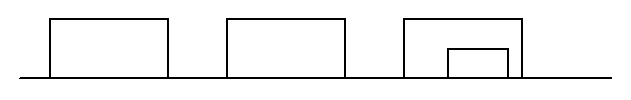
\includegraphics[scale=1.0]{substring-search.9.eps} \\
~\\
~\\
Пересекающиеся: \\
\includegraphics[scale=1.0]{substring-search.10.eps}
}

\frame{
  \frametitle{Непересечение интервалов}
  \begin{rtheorem}
    Никакие два покрытых интервала, вычисленных алгоритмом, не
    пересекаются. Более того, если алгоритм проверяет позицию $h$ из
    $T$ в покрытом интервале, то $h$ --- правый конец этого
    интервала. 
  \end{rtheorem}
}
\frame{
  \frametitle{Непересечение интервалов: доказательство}
  \begin{proof}
    \begin{itemize}
    \item Индукция по количеству интервалов. 
    \item Перемещение $h$ внутрь интервала возможно только в случаях 2 или 5, но
      тогда будет нарушено индукционное предположение.
    \item Новый интервал $[h+1..j]$ создаётся в случаях 1 ($h$ не
      принадлежит ни одному интервалу), 3 и 4 ($h$ --- правый конец
      интервала), следовательно он не пересекает существующих интервалов. 
    \end{itemize}
  \end{proof}
}

\frame{
  \frametitle{Линейность алгоритма}
  \begin{rtheorem}
    Алгоритм Апостолико-Джанкарло выполняет не более $2m$ сравнений
    символов и не более $O(m)$ дополнительных действий. 
  \end{rtheorem}
  \begin{proof}
    \begin{itemize}
      \item Количество несовпадений $\leq m$ (завершение фазы и сдвиг.)
      \item Символы сравниваются в случае 1, результаты совпадений
        заносятся в $M(j)$, т.е. эти символы попадают в  интервал. 
      \item Символы внутри покрытых интервалов не сравниваются,
        т.е. $m$ совпадений и $2m$ сравнений. 
      \item Количество обращений к $M$ имеет порядок $O(M)$, т.к. в
        случаях 3 и 4 происходит сдвиг, а в случаях 2 и 5 создастся
        новый интервал.
    \end{itemize}
  \end{proof}
}

\frame{
  \frametitle{Выводы}
  \begin{itemize}
    \item Алгоритм полностью имитирует алгоритм Бойера-Мура. 
    \item За счёт сохранения накопленной в процессе сравнивания
      образца с текстом пропускаются некоторые сравнения. 
    \item Простая линейная оценка. 
  \end{itemize}
}

%\subsection{Классический вариант алгоритма}

\end{document}
    
